\documentclass[aspectratio=169,10pt,t]{beamer}

% ---- engine-safe fonts ---------------------------------------------
\usepackage{iftex}
\ifPDFTeX
  \usepackage[T1]{fontenc}
  \usepackage[utf8]{inputenc}
  \usepackage[scaled=0.92]{helvet}
\else
  \usepackage{fontspec}
\fi
\renewcommand{\familydefault}{\sfdefault}

\usepackage{tikz}
\usetikzlibrary{arrows.meta,positioning,calc,shapes.geometric,decorations.pathreplacing}
\usepackage[most]{tcolorbox}
\usepackage{booktabs}
\usepackage{amsmath,amssymb,mathtools}
\usepackage{graphicx}

% =====================================================================
%  THEME
% =====================================================================
\usetheme{default}
\usecolortheme{default}
\setbeamertemplate{navigation symbols}{}

\definecolor{calblue}{HTML}{003262}
\definecolor{calgold}{HTML}{FDB515}
\definecolor{ink}{HTML}{1C1C1E}
\definecolor{muted}{HTML}{8A8F98}
\definecolor{softbg}{HTML}{F4F6F8}
\definecolor{signal}{HTML}{A8322D}
\definecolor{good}{HTML}{2E6B4F}

\setbeamercolor{normal text}{fg=ink,bg=white}
\setbeamercolor{structure}{fg=calblue}
\setbeamercolor{frametitle}{fg=calblue,bg=}
\setbeamercolor{framesubtitle}{fg=muted}
\setbeamerfont{frametitle}{size=\Large,series=\bfseries}
\setbeamerfont{framesubtitle}{size=\small,series=\mdseries}

\setbeamersize{text margin left=0.045\paperwidth,
               text margin right=0.045\paperwidth}

% ---- frame title ----------------------------------------------------
\makeatletter
\setbeamertemplate{frametitle}{%
  \vspace*{0.7em}%
  \begin{minipage}{\textwidth}
    \raggedright
    \setlength{\parskip}{0pt}%
    {\usebeamerfont{frametitle}\usebeamercolor[fg]{frametitle}\insertframetitle\par}%
    \ifx\insertframesubtitle\@empty\else
      \vspace*{-0.10em}%
      {\usebeamerfont{framesubtitle}\usebeamercolor[fg]{framesubtitle}\insertframesubtitle\par}%
    \fi
    \vspace*{-0.55em}%
    {\color{calgold}\rule{2.4em}{2pt}}%
  \end{minipage}%
  \vspace*{0.30em}%
}
\makeatother

\setbeamertemplate{footline}{%
  \hspace*{0.045\paperwidth}%
  \parbox[b]{0.91\paperwidth}{%
    \color{muted}\scriptsize
    \hfill\insertframenumber
  }%
  \vspace{1.1em}
}

% list markers
\setbeamertemplate{itemize item}{\color{calgold}\rule[0.33ex]{0.42em}{0.42em}}
\setbeamertemplate{itemize subitem}{\color{muted}\textendash}
\setbeamertemplate{enumerate item}{\color{calblue}\bfseries\insertenumlabel.}
\setlength{\leftmargini}{1.3em}
\setlength{\leftmarginii}{1.1em}

% ---- boxes ----------------------------------------------------------
\newtcolorbox{goldbox}{enhanced,sharp corners,boxrule=0pt,leftrule=3pt,
  colframe=calgold,colback=softbg,
  left=9pt,right=9pt,top=4pt,bottom=4pt,before skip=3pt,after skip=3pt}

\newtcolorbox{bluebox}{enhanced,sharp corners,boxrule=0pt,leftrule=3pt,
  colframe=calblue,colback=softbg,
  left=9pt,right=9pt,top=4pt,bottom=4pt,before skip=3pt,after skip=3pt}

\newtcolorbox{signalbox}{enhanced,sharp corners,boxrule=0pt,leftrule=3pt,
  colframe=signal,colback=signal!5,
  left=9pt,right=9pt,top=4pt,bottom=4pt,before skip=3pt,after skip=3pt}

\newtcolorbox{goodbox}{enhanced,sharp corners,boxrule=0pt,leftrule=3pt,
  colframe=good,colback=good!5,
  left=9pt,right=9pt,top=4pt,bottom=4pt,before skip=3pt,after skip=3pt}

% ---- shorthands -----------------------------------------------------
\newcommand{\key}[1]{\textcolor{calblue}{\textbf{#1}}}
\newcommand{\hi}[1]{\textbf{#1}}
\newcommand{\quiet}[1]{\textcolor{muted}{#1}}
\newcommand{\warn}[1]{\textcolor{signal}{\textbf{#1}}}
\newcommand{\thinrule}{\vspace{0.4em}{\color{muted!40}\hrule}\vspace{0.5em}}

% ---- reclaim vertical space without scaling the frame ----------------
\newcommand{\tightmath}{%
  \setlength{\abovedisplayskip}{3pt}%
  \setlength{\belowdisplayskip}{3pt}%
  \setlength{\abovedisplayshortskip}{1pt}%
  \setlength{\belowdisplayshortskip}{1pt}%
}

% ---- missing-figure guard -------------------------------------------
\newcommand{\safegraphic}[2][width=\textwidth]{%
  \IfFileExists{#2}%
    {\includegraphics[#1]{#2}}%
    {
\begin{tikzpicture}
       \fill[softbg] (0,0) rectangle (11,5.2);
       \draw[muted!40,line width=0.6pt] (0,0) rectangle (11,5.2);
       \node[text=muted,font=\small\ttfamily] at (5.5,2.6) {\detokenize{#2}};
     \end{tikzpicture}}%
}

% ---- title page -----------------------------------------------------
\setbeamertemplate{title page}{%
  \vspace{1.4em}
  {\color{calgold}\rule{3em}{2.5pt}}\par
  \vspace{1.0em}
  {\color{white}\fontsize{22}{26}\selectfont\bfseries\inserttitle\par}
  \vspace{0.7em}
  {\color{calgold}\large\insertsubtitle\par}
  \vspace{2.2em}
  {\color{white!85}\small\insertauthor\par}
  \vspace{0.35em}
  {\color{white!55}\footnotesize\insertinstitute\ \textperiodcentered\ \insertdate\par}
}

% ---- additions --------------------------------------------------------
\newcommand{\tightlines}{\linespread{0.92}\selectfont}
% coloured tokens for the opening slide (green list / red list), dark text on light fill
\newcommand{\gtok}[1]{{\setlength{\fboxsep}{0.8pt}\colorbox{good!16}{\strut\textcolor{good!70!black}{#1}}}}
\newcommand{\rtok}[1]{{\setlength{\fboxsep}{0.8pt}\colorbox{signal!13}{\strut\textcolor{signal!80!black}{#1}}}}
\newcommand{\ptok}[1]{{\setlength{\fboxsep}{0.8pt}\colorbox{white}{\strut #1}}}   % same box, uncoloured (plain overlay)
% TikZ styles for the small pipeline diagrams
\tikzset{
  stepbox/.style = {rectangle, draw=calblue, line width=0.8pt, fill=softbg, rounded corners=1pt,
                    minimum height=7mm, inner sep=3pt, font=\scriptsize, align=center},
  flow/.style    = {-{Latex[length=1.8mm]}, line width=0.8pt, draw=calblue},
  lbl/.style     = {font=\scriptsize, text=muted}
}
% live-demo slide: title only + placeholder that becomes the screenshot once figures/<file> exists
\newcommand{\demoframe}[2]{%
  \begin{frame}{#1}
    \vspace{0.6em}
    \begin{center}\safegraphic[width=0.94\textwidth,height=0.70\paperheight,keepaspectratio]{figures/#2}\end{center}
    \note{Switch to the browser for the live page.}
  \end{frame}}

\title[A Watermark for Large Language Models]{A Watermark for Large Language Models}
\subtitle{Kirchenbauer et al. -- University of Maryland, ICML 2023 \textperiodcentered\ Reproduction and extensions}
\author{Romain Almeida \textperiodcentered \ Piero Pelosi \textperiodcentered \ Elias Roubache}
\institute{MFE 230ZB Generative AI and Causality \textperiodcentered\ Prof. Ali Kakhbod}
\date{October 2026}

\begin{document}
% generated by make_figures.py: AI email = sample 11 of 16 from Qwen/Qwen2.5-1.5B-Instruct with the watermark (gamma 0.25, delta 2, temperature 0.7), snippets/emails.json; human email = EMAIL_HUMAN in make_figures.py
\newcommand{\emailHumanPlain}{Subject: Zoom meeting for our fall project\par\vspace{0.35em}Hi Professor Kakhbod,\par\vspace{0.35em}Romain, Elias and I picked the watermarking paper for our fall project. Could we grab 20 minutes on Zoom to run our plan by you before we start the experiments? Thursday afternoon or Friday morning both work for us, but we can adapt to your schedule.\par\vspace{0.35em}Thanks a lot,\newline Piero}
\newcommand{\emailHumanColor}{\gtok{Subject}\rtok{:} \gtok{Zoom} \rtok{meeting} \rtok{for} \rtok{our} \rtok{fall} \rtok{project}\gtok{\ensuremath{\hookleftarrow}} \rtok{Hi} \rtok{Professor} \gtok{K}\rtok{akh}\gtok{b}\rtok{od}\rtok{,}\rtok{\ensuremath{\hookleftarrow}} \gtok{R}\rtok{omain}\rtok{,} \rtok{Elias} \rtok{and} \gtok{I} \rtok{picked} \rtok{the} \rtok{watermark}\rtok{ing} \gtok{paper} \rtok{for} \rtok{our} \rtok{fall} \rtok{project}\rtok{.} \gtok{Could} \gtok{we} \rtok{grab}\rtok{2}\rtok{0} \rtok{minutes} \gtok{on} \rtok{Zoom} \rtok{to} \rtok{run} \rtok{our} \gtok{plan} \rtok{by} \gtok{you} \rtok{before} \rtok{we} \rtok{start} \rtok{the} \rtok{experiments}\rtok{?} \gtok{Thursday} \rtok{afternoon} \gtok{or} \gtok{Friday} \rtok{morning} \rtok{both} \rtok{work} \gtok{for} \rtok{us}\rtok{,} \rtok{but} \rtok{we} \rtok{can} \rtok{adapt} \rtok{to} \gtok{your} \rtok{schedule}\rtok{.}\rtok{\ensuremath{\hookleftarrow}} \gtok{Thanks} \rtok{a} \gtok{lot}\rtok{,}\rtok{\ensuremath{\hookleftarrow}} \gtok{P}\rtok{iero}}
\newcommand{\emailHumanTokens}{77}
\newcommand{\emailHumanGreen}{21}
\newcommand{\emailHumanExpected}{19}
\newcommand{\emailHumanZ}{0.5}
\newcommand{\emailAIPlain}{Subject: Request for Fall Project Meeting\par\vspace{0.35em}Dear Professor Kakhbod,\par\vspace{0.35em}I hope this message finds you well.\par\vspace{0.35em}As an MFE student at UC Berkeley and part of your research group, I would like to request a zoom meeting sometime next week to discuss our upcoming fall project. Our topic is [insert topic] with current progress being discussed in class. Would there be any availability after [insert date and time]?\par\vspace{0.35em}Thank you very much for your time and consideration.\par\vspace{0.35em}Best regards,\newline Piero}
\newcommand{\emailAIColor}{\gtok{Subject}\rtok{:} \gtok{Request} \rtok{for} \rtok{Fall} \rtok{Project} \rtok{Meeting}\rtok{\ensuremath{\hookleftarrow}} \gtok{Dear} \rtok{Professor} \gtok{K}\rtok{akh}\gtok{b}\rtok{od}\rtok{,}\rtok{\ensuremath{\hookleftarrow}} \rtok{I} \rtok{hope} \rtok{this} \rtok{message} \rtok{finds} \rtok{you} \gtok{well}\gtok{.}\gtok{\ensuremath{\hookleftarrow}} \gtok{As} \rtok{an} \rtok{M}\gtok{FE} \rtok{student} \rtok{at} \rtok{UC} \rtok{Berkeley} \gtok{and} \rtok{part} \rtok{of} \gtok{your} \gtok{research} \rtok{group}\gtok{,} \rtok{I} \rtok{would} \rtok{like} \gtok{to} \gtok{request} \gtok{a} \gtok{zoom} \rtok{meeting} \gtok{sometime} \rtok{next} \rtok{week} \rtok{to} \rtok{discuss} \rtok{our} \gtok{upcoming} \gtok{fall} \rtok{project}\rtok{.} \rtok{Our} \gtok{topic} \rtok{is} \gtok{[}\gtok{insert} \rtok{topic}\gtok{]} \gtok{with} \gtok{current} \rtok{progress} \gtok{being} \rtok{discussed} \rtok{in} \gtok{class}\rtok{.} \gtok{Would} \gtok{there} \gtok{be} \gtok{any} \gtok{availability} \gtok{after} \gtok{[}\gtok{insert} \rtok{date} \rtok{and} \gtok{time}\gtok{]?}\gtok{\ensuremath{\hookleftarrow}} \rtok{Thank} \rtok{you} \gtok{very} \rtok{much} \gtok{for} \gtok{your} \gtok{time} \rtok{and} \rtok{consideration}\gtok{.}\gtok{\ensuremath{\hookleftarrow}} \gtok{Best} \rtok{regards}\gtok{,}\gtok{\ensuremath{\hookleftarrow}} \gtok{P}\rtok{iero}}
\newcommand{\emailAITokens}{99}
\newcommand{\emailAIGreen}{47}
\newcommand{\emailAIExpected}{25}
\newcommand{\emailAIZ}{5.2}
\newcommand{\emailAIOdds}{1 in 8 million}
\newcommand{\emailSamples}{16}
\newcommand{\emailSamplesAbove}{12}
\newcommand{\emailSamplesMedian}{4.8}


{
\setbeamercolor{background canvas}{bg=calblue}
\begin{frame}[plain]
  \titlepage
  \note{Kirchenbauer, Geiping, Wen, Katz, Miers, Goldstein, A Watermark for Large Language Models, ICML 2023 (arXiv 2301.10226).
  Plan: the paper (10 minutes with three live demos), our reproduction, four extensions, takeaways.}
\end{frame}
}

% =====================================================================
%  THE PAPER
% =====================================================================

% ---- 2 ----------------------------------------------------------------
\begin{frame}{Two emails to Professor Kakhbod}
  To book a Zoom meeting about our fall project, I emailed Professor Kakhbod. Here are two versions.
  \vspace{0.2em}

  \begin{columns}[T,onlytextwidth]
    \begin{column}{0.49\textwidth}
      \begin{tcolorbox}[enhanced,sharp corners,boxrule=0.4pt,colframe=muted!35,colback=white,borderline west={3pt}{0pt}{calblue},left=8pt,right=8pt,top=4pt,bottom=4pt,before skip=3pt,after skip=3pt,equal height group=emails]
        \key{A}\par\vspace{0.2em}
        {\small\raggedright\emailHumanPlain\par}
      \end{tcolorbox}
    \end{column}
    \begin{column}{0.49\textwidth}
      \begin{tcolorbox}[enhanced,sharp corners,boxrule=0.4pt,colframe=muted!35,colback=white,borderline west={3pt}{0pt}{calblue},left=8pt,right=8pt,top=4pt,bottom=4pt,before skip=3pt,after skip=3pt,equal height group=emails]
        \key{B}\par\vspace{0.2em}
        {\small\raggedright\emailAIPlain\par}
      \end{tcolorbox}
    \end{column}
  \end{columns}
  \vspace{1.2em}

  {\centering\large One of them I wrote with AI. \key{Which one?}\par}
  \note{Show of hands: A or B? Expect a split vote: that is the point. Models now write like us, which is the classifier's problem on the next slide.
  B is real output of Qwen2.5-1.5B-Instruct with our watermark (gamma 0.25, delta 2, temperature 0.7), given the same points as A (chosen paper, 20 minutes on Zoom, Thursday or Friday) and told to write plainly; sample 44 of \emailSamples, picked because it reads like a student wrote it (snippets/emails.json). Its slip, ``your paper'', is the model's. A is the human email (EMAIL\_HUMAN in make\_figures.py). The side was drawn at random.}
\end{frame}

% ---- 3 ----------------------------------------------------------------
\begin{frame}{How would Professor Kakhbod catch me?}
  \framesubtitle{The paper}
  The naive approach: train a \key{classifier} on human vs AI text. Three problems:
  \begin{itemize}
    \item no guarantee and no known error rate;
    \item it degrades as models improve;
    \item it accuses humans.
  \end{itemize}
  \vspace{0.8em}
  \begin{center}
  \begin{tabular}{@{}lcc@{}}
    \toprule
     & AI text caught & human text flagged as AI \\
    \midrule
    OpenAI AI Text Classifier (January 2023) & 26\% & 9\% \\
    \bottomrule
  \end{tabular}
  \end{center}
  \vspace{0.6em}
  \quiet{\small OpenAI withdrew its classifier in July 2023 for its low rate of accuracy.}
  \note{OpenAI blog, ``New AI classifier for indicating AI-written text'' (31 Jan 2023, updated 20 Jul 2023): 26\% true positives, 9\% false positives on their challenge set; withdrawn for low accuracy.
  Talking point: the vote just showed problem 2, models now write like humans. With 9\% false positives, Professor Kakhbod would also wrongly accuse about one honest email in eleven.
  The paper's numbers come on the next slide.}
\end{frame}

% ---- 4 ----------------------------------------------------------------
\begin{frame}{The paper's idea: a watermark}
  \framesubtitle{The paper}
  \begin{columns}[T,onlytextwidth]
    \begin{column}{0.44\textwidth}
      \raggedright
      \begin{goldbox}
        \raggedright A \key{watermark} is ``a hidden pattern in text that is imperceptible to humans, while making the text algorithmically identifiable as synthetic.''
      \end{goldbox}
      \vspace{0.4em}
      The model owner adds it while the model writes. Anyone holding the key can check. Nothing is retrained.
    \end{column}
    \begin{column}{0.51\textwidth}
      \key{Five properties}
      \begin{enumerate}
        \item Detectable without the model or its API.
        \item Works on any existing model, no retraining.
        \item Detectable from any contiguous slice of text.
        \item Cannot be removed without changing a large share of the tokens.
        \item Comes with a rigorous p-value.
      \end{enumerate}
    \end{column}
  \end{columns}
  \vspace{0.7em}
  \begin{center}
  \small
  \begin{tabular}{@{}lcc@{}}
    \toprule
     & AI text caught & human text flagged as AI \\
    \midrule
    OpenAI AI Text Classifier (2023) & 26\% & 9\% \\
    \key{Watermark}, at the paper's threshold $z = 4$ & \key{98.4\%} & \key{about 0.003\%} (3 in 100{,}000) \\
    \bottomrule
  \end{tabular}
  \end{center}
  \note{Definition quoted from the paper's introduction; the five properties are the paper's list (Sec. 1).
  Table: OpenAI blog (slide 3). Watermark: 98.4\% is the paper's detection rate at z = 4 on 200-token texts (Sec. 4.1, gamma 0.5, delta 2); 0.003\% is the one-sided p-value at z = 4 (3.2e-5), a false-alarm rate fixed by the test, not estimated.
  The difference: the watermark is put in on purpose while the model writes, so the test knows exactly what to look for.}
\end{frame}

% ---- 5 ----------------------------------------------------------------
\begin{frame}{Back to my emails, in colour}
  \framesubtitle{The paper}
  \begin{columns}[T,onlytextwidth]
    \begin{column}{0.35\textwidth}
      \raggedright\small
      \begin{enumerate}
        \item A secret key colours every token \gtok{green} or \rtok{red}, based on the token before it. A quarter of the vocabulary is green.
        \item A human does not know the key, so their tokens land on green only by luck: about 1 in 4.
        \item The AI was pushed toward green while writing, so green piles up.
      \end{enumerate}
      \vspace{0.2em}
      \begin{goldbox}
        \raggedright B: \emailAIGreen\ green where chance gives \emailAIExpected, $z = \emailAIZ$. By chance: \emailAIOdds.
      \end{goldbox}
    \end{column}
    \begin{column}{0.62\textwidth}
      \begin{tcolorbox}[enhanced,sharp corners,boxrule=0.4pt,colframe=muted!35,colback=white,borderline west={3pt}{0pt}{calblue},left=7pt,right=7pt,top=3pt,bottom=3pt,before skip=0pt,after skip=4pt]
        {\footnotesize\key{A}\quad green tokens: \emailHumanGreen\ of \emailHumanTokens, chance gives \emailHumanExpected\hfill{\scriptsize\quiet{$\hookleftarrow$ = line break, a token too}}}\par\vspace{0.15em}
        {\scriptsize\raggedright\emailHumanColor\par}
      \end{tcolorbox}
      \begin{tcolorbox}[enhanced,sharp corners,boxrule=0.4pt,colframe=muted!35,colback=white,borderline west={3pt}{0pt}{calblue},left=7pt,right=7pt,top=3pt,bottom=3pt,before skip=0pt,after skip=3pt]
        {\footnotesize\key{B}\quad green tokens: \emailAIGreen\ of \emailAITokens, chance gives \emailAIExpected}\par\vspace{0.15em}
        {\scriptsize\raggedright\emailAIColor\par}
      \end{tcolorbox}
      \vspace{0.3em}
      {\footnotesize\raggedright\quiet{Since August 2026, Anthropic watermarks Claude's text with a scheme from this family (a version of SynthID-Text).}\par}
    \end{column}
  \end{columns}
  \note{Colours are real: the detector run on both emails with the Qwen tokenizer and our key, gamma = 0.25 (snippets/emails.tex, made by make\_figures.py). The first token's context is the end of the chat prompt.
  A (mine): \emailHumanGreen\ green of \emailHumanTokens\ tokens, z = \emailHumanZ. B (AI, delta = 2): \emailAIGreen\ of \emailAITokens, z = \emailAIZ, one-sided p-value: \emailAIOdds.
  Honest caveat if asked: detection is not guaranteed on text this short. \emailSamplesAbove\ of the \emailSamples\ AI samples exceed z = 4 (median z \emailSamplesMedian); we showed one that reads naturally and is detected. Short text is exactly Extension 1.
  Tokens are words or pieces of words: ``Kakhbod'' is four tokens. Anthropic line: from Anthropic's public statement, as given in the brief.}
\end{frame}

% ---- 6 ----------------------------------------------------------------
\begin{frame}{Algorithm 1: ban half the vocabulary}
  \framesubtitle{The paper \textperiodcentered\ Algorithm 1}
  \begin{center}
  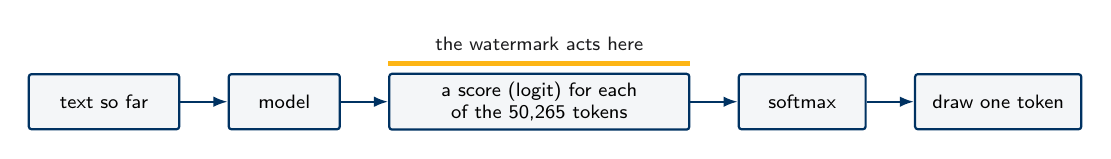
\begin{tikzpicture}[node distance=6mm]
    \node[stepbox, text width=17mm] (a) {text so far};
    \node[stepbox, text width=12mm, right=of a] (b) {model};
    \node[stepbox, text width=36mm, right=of b] (c) {a score (logit) for each\\of the 50{,}265 tokens};
    \node[stepbox, text width=14mm, right=of c] (d) {softmax};
    \node[stepbox, text width=19mm, right=of d] (e) {draw one token};
    \draw[flow] (a) -- (b);
    \draw[flow] (b) -- (c);
    \draw[flow] (c) -- (d);
    \draw[flow] (d) -- (e);
    \draw[calgold, line width=2pt] ($(c.north west)+(0,1.2mm)$) -- ($(c.north east)+(0,1.2mm)$);
    \node[font=\scriptsize, text=ink, above=1.6mm of c] {the watermark acts here};
  \end{tikzpicture}
  \end{center}
  \vspace{-0.7em}
  \begin{columns}[T,onlytextwidth]
    \begin{column}{0.52\textwidth}
      \begin{bluebox}
        \small\raggedright
        \key{Algorithm 1}, at every step $t$:
        \begin{enumerate}
          \item run the model: probabilities $p^{(t)}$;
          \item hash the previous token $s^{(t-1)}$ with a secret key into a seed;
          \item with that seed, split the vocabulary into a \textcolor{good}{\textbf{green}} and a \textcolor{signal}{\textbf{red}} half;
          \item ban red: sample $s^{(t)}$ from the green half.
        \end{enumerate}
      \end{bluebox}
      {\small\raggedright The previous token fixes the split: with the key, anyone can rebuild every list from the text alone, without the model.\par}
    \end{column}
    \begin{column}{2.75in}
      \vspace{-0.3em}
      \safegraphic[width=\linewidth]{figures/ban_dinner.pdf}
    \end{column}
  \end{columns}
  \note{Figure: illustrative probabilities (six equally good dishes, three green); under the ban each green dish goes from 1/6 to 1/3 and the red ones to 0. Plenty of good options, so banning half costs nothing here.
  OPT-1.3B vocabulary: 50,265 tokens. In the code: seed = 15,485,863 x previous token id; green list = first gamma N entries of a seeded random permutation of the vocabulary; context width h = 1.
  Algorithm 1 is the gamma = 0.5 case with red tokens at probability zero.}
\end{frame}

% ---- 7 ----------------------------------------------------------------
\begin{frame}{Detection is a count against chance}
  \framesubtitle{The paper \textperiodcentered\ Algorithm 1}
  \begin{columns}[T,onlytextwidth]
    \begin{column}{0.50\textwidth}
      \raggedright
      \key{$H_0$}: the text was written without knowing the lists (a human, or another model). Then each token is green with probability $1/2$:
      \[ |s|_G \sim \mathrm{Binomial}(T, 1/2), \qquad z = \frac{2\,(|s|_G - T/2)}{\sqrt{T}} \]
      $|s|_G$: green tokens among the $T$ tested. Flag the text if $z > 4$: one-sided p-value $3.2\times10^{-5}$.
      \vspace{0.3em}
      \begin{goldbox}
        \raggedright
        All green: $z = \sqrt{T}$, so \hi{16 tokens} already reach $z = 4$.\par\vspace{0.2em}
        Edit 200 of 1{,}000 tokens: at most 400 red, still $z \approx 6.3$.
      \end{goldbox}
    \end{column}
    \begin{column}{2.75in}
      \safegraphic[width=\linewidth]{figures/z_null.pdf}
    \end{column}
  \end{columns}
  \note{Figure: the z-scores of our 1,000 human texts (C4, gamma 0.5, our key, results/raw/human/c4) against the standard normal curve of chance: mean -0.20, sd 1.04, none above 4. The threshold z = 4 leaves a tail of 3.2e-5 (1 - Phi(4)).
  Detection needs only the text and the key: no model, no API (property 1).
  16 green tokens give z = 4 exactly; one more passes the strict threshold.
  Attack arithmetic is the paper's Sec. 2 example: each edit can also turn the next token red, so 200 edits make at most 400 red tokens; 600 green of 1,000 gives z = 200/sqrt(1000) = 6.3.
  A high count means ``this watermark is here''; a low count proves nothing.}
\end{frame}

% ---- 8 ----------------------------------------------------------------
\demoframe{Live: the hard red list}{demo_algo1.png}

% ---- 9 ----------------------------------------------------------------
\begin{frame}{Where the hard rule breaks}
  \framesubtitle{The paper \textperiodcentered\ Algorithm 1}
  \begin{columns}[T,onlytextwidth]
    \begin{column}{0.50\textwidth}
      \raggedright
      \key{Low-entropy text}: the next token is almost forced.
      \begin{itemize}
        \item After ``Barack'' the model puts about 99\% on ``Obama''. If ``Obama'' is red, the ban forces ``Hussein'' or ``and''.
        \item Same for code, \texttt{for(i=0;i<n;i++)}, and for memorised quotes.
      \end{itemize}
      \vspace{0.2em}
      \begin{signalbox}
        \raggedright
        \warn{Two problems}
        \begin{enumerate}
          \item Humans and models write the same thing there, so no test can tell them apart.
          \item Forcing a different token wrecks the text.
        \end{enumerate}
      \end{signalbox}
      So the authors replace the ban by a push.
    \end{column}
    \begin{column}{2.75in}
      \safegraphic[width=\linewidth]{figures/ban_barack.pdf}
    \end{column}
  \end{columns}
  \note{Figure: same illustrative inputs as the push example on slide 12 (Obama 0.990, red): the ban sends Obama to 0 and gives Hussein 0.571 and and 0.429. Compare slide 6: with many good options the ban was harmless; with one, it breaks the sentence.
  Low entropy means a spiked next-token distribution. Both problems are from the paper's Sec. 2 and 3: detectability and quality.}
\end{frame}

% ---- 10 ---------------------------------------------------------------
\demoframe{Live: Barack $\to$ Obama}{demo_barack.png}

% ---- 11 ---------------------------------------------------------------
\begin{frame}{Algorithm 2: from a ban to a push}
  \framesubtitle{The paper \textperiodcentered\ Algorithm 2}
  \tightmath
  \begin{bluebox}
    \key{Algorithm 2}, at every step $t$: steps 1 to 3 unchanged.\par
    Step 4: add $\delta$ to the logit of every green token, $\tilde l_k = l_k + \delta\,\mathbf{1}\{k \in G_t\}$, then softmax and sample.
  \end{bluebox}
  \vspace{0.3em}
  With $\alpha = e^{\delta}$ and $p_G = \sum_{k \in G_t} p_k$, the model's own probability on green tokens:
  \[ \Pr(\text{green}) = \frac{\alpha\,p_G}{1+(\alpha-1)\,p_G} \]
  The odds of writing a green token are multiplied by $e^{\delta}$ ($\times 7.4$ at $\delta = 2$). Red tokens stay allowed.
  \vspace{0.5em}
  \begin{center}
  \begin{tabular}{@{}lll@{}}
    \toprule
    knob & meaning & paper \\
    \midrule
    $\gamma$ & green share of the vocabulary & 0.25 or 0.5 \\
    $\delta$ & strength of the push & 2 (main value) \\
    \bottomrule
  \end{tabular}
  \end{center}
  \note{The formula follows from the softmax: green logits shifted by delta multiply green probabilities by alpha before renormalising.
  Odds form: Pr(green)/(1 - Pr(green)) = alpha p\_G/(1 - p\_G). e\^{}2 = 7.39.
  With gamma = 0.5 the green list is half the vocabulary; gamma = 0.25 a quarter.
  In the paper's code delta is added before the temperature 0.7 (we checked the same order in transformers; backup B7).}
\end{frame}

% ---- 12 ---------------------------------------------------------------
\begin{frame}{The push only acts where the model has a choice}
  \framesubtitle{The paper \textperiodcentered\ Algorithm 2}
  \vspace{0.2em}
  \safegraphic[width=\linewidth]{figures/push_example.pdf}
  \vspace{0.3em}

  Confident model: the push changes almost nothing, so quality is kept. Several good options: the push decides, so green tokens pile up.
  \note{Illustrative numbers, not measured: the model probabilities are made up, the watermarked ones are computed with the slide-11 formula at delta = 2 (make\_figures.py, push\_example). Same inputs as the ban figures on slides 6 and 9.
  Left: Obama is red, 0.990 to 0.948; the chance of a green token goes from 0.7\% to 5\%.
  Right: six equally good words, three green: each green word 0.167 to 0.294, each red 0.167 to 0.040; green chance 50\% to 88\%.
  This is why the soft watermark keeps quality and still leaves a signal where there is choice.}
\end{frame}

% ---- 13 ---------------------------------------------------------------
\begin{frame}{Detection: the same count, for any $\gamma$}
  \framesubtitle{The paper \textperiodcentered\ Algorithm 2}
  \tightmath
  \[ z = \frac{|s|_G - \gamma T}{\sqrt{T\,\gamma(1-\gamma)}} = \sqrt{T}\,\frac{f - \gamma}{\sqrt{\gamma(1-\gamma)}}, \qquad f = \text{green fraction} \]
  At a fixed green fraction, evidence grows like $\sqrt{T}$ (law of large numbers plus the normal approximation).
  \vspace{0.5em}

  Paper's main setting ($T = 200$, $\gamma = 0.5$, $\delta = 2$):
  \begin{itemize}
    \item human text has $100 \pm 7$ green tokens;
    \item $z = 4$ corresponds to about 128 green tokens;
    \item watermarked texts average 159.5, so $z \approx 8.4$.
  \end{itemize}
  \vspace{0.3em}
  \begin{goldbox}
    $z$ depends only on $\gamma$ and the key, not on $\delta$: the push can vary by context behind one detector.
  \end{goldbox}
  \note{100 +/- 7: mean gamma T = 100, sd sqrt(200 x 0.25) = 7.07.
  z = 4 at 100 + 4 x 7.07 = 128.3 green tokens (129 to exceed it strictly).
  159.5 is the paper's observed mean (Sec. 4.1): z = 59.5/7.07 = 8.4.
  The detector never needs delta: a deployer can change the strength by context without changing detection.}
\end{frame}

% ---- 14 ---------------------------------------------------------------
\begin{frame}{Theorem 4.2: how many green tokens to expect}
  \framesubtitle{The paper \textperiodcentered\ Algorithm 2}
  \tightmath
  \begin{goldbox}
    \vspace{-0.3em}
    \[ \mathbb{E}\,|s|_G \;\ge\; T \cdot \frac{\gamma\,\alpha}{1+(\alpha-1)\gamma} \cdot S^\star \]
    $S^\star$: the average ``spread'' of the model's next-token choices along the text (the paper's spike entropy, defined in backup). The theorem also bounds the variance.
  \end{goldbox}
  \vspace{0.5em}
  \begin{columns}[T,onlytextwidth]
    \begin{column}{0.55\textwidth}
      \key{Three factors}
      \begin{enumerate}
        \item the length $T$;
        \item the best green rate the push reaches when the model is indifferent: 0.88 at $\gamma = 0.5$, $\delta = 2$;
        \item how often the model actually has a choice.
      \end{enumerate}
      No choice at all: the bound falls to $\gamma T$, what a human gets by chance.
    \end{column}
    \begin{column}{0.41\textwidth}
      \vspace{0.2em}
      {\small
      \begin{tabular}{@{}lr@{}}
        \toprule
        Paper, \S 4.1 ($T = 200$) & \\
        \midrule
        average spread & 0.807 \\
        bound on green tokens & 142.2 \\
        observed & 159.5 \\
        predicted detection, $z = 4$ & $\ge 98.6\%$ \\
        observed detection & 98.4\% \\
        \bottomrule
      \end{tabular}}
    \end{column}
  \end{columns}
  \note{0.88 = gamma alpha/(1 + (alpha - 1) gamma) at gamma 0.5, alpha = e\^{}2: 0.881.
  At the lowest spread, S = (1 + (alpha - 1) gamma)/alpha, the bound is exactly gamma T.
  The observed 98.4\% is below the predicted 98.6\% because the prediction is for a text at average entropy; the misses are low-entropy texts (100\% detected above the 25th entropy percentile).
  Definition of spike entropy and the variance bound: backup B1.}
\end{frame}

% ---- 15 ---------------------------------------------------------------
\demoframe{Live: the soft watermark}{demo_algo2.png}

% ---- 16 ---------------------------------------------------------------
\begin{frame}{What the soft watermark leaves open}
  \framesubtitle{The paper}
  \vspace{0.4em}
  \begin{tabular}{@{}p{0.34\textwidth}p{0.44\textwidth}l@{}}
    \toprule
    Limit & Why & What we test \\
    \midrule
    \raggedright Constrained text (code, short factual answers) & \raggedright little choice, little signal & Extension 1 \\[0.3em]
    \raggedright A modern rewrite & \raggedright the paper attacks with T5 word swaps (2020) & Extension 2 \\[0.3em]
    \raggedright A watermarked passage pasted into human text & \raggedright the paper's conclusion lists it as open & Extension 3 \\[0.3em]
    \raggedright Side effects of the key itself & \raggedright the key fixes the colour of every token pair, ``stop'' included & Extension 4 \\
    \bottomrule
  \end{tabular}
  \vspace{1em}

  \quiet{Repeated phrases get the same colour every time, which breaks the independence the test assumes (\hyperlink{b2}{backup B2}, \hyperlink{b14}{B14}).}
  \note{These four limits structure the second half of the talk.
  Extension 1 follows from Theorem 4.2 itself; Extension 2 updates the attacker; Extension 3 answers the paper's open question with the authors' own later tool; Extension 4 is a side effect we found.
  Repetition: the paper's Appendix B suggests counting each repeated pair once.}
\end{frame}

% =====================================================================
%  REPRODUCTION
% =====================================================================

% ---- 17 ---------------------------------------------------------------
\begin{frame}{Same experiments, our own code}
  \framesubtitle{Reproduction}
  {\small
  \begin{tabular}{@{}p{0.15\textwidth}p{0.41\textwidth}p{0.37\textwidth}@{}}
    \toprule
     & Paper & Ours \\
    \midrule
    Texts & \raggedright C4 news articles: start = prompt, last 200 tokens = human text & \raggedright same \tabularnewline
    Writing model & OPT-1.3B & same \\
    Settings & \raggedright $\tau = 0.7$, $T = 200 \pm 5$, $\gamma$ and $\delta$ grids, multinomial and beam search & \raggedright same \tabularnewline
    Quality judge & OPT-2.7B perplexity & same \\
    Sample & \raggedright about 500 texts per setting & \raggedright 100 to 500 per setting (497 for the headline), plus 1{,}000 human texts \tabularnewline
    Attack & \raggedright T5-Large span replacement (code never released) & \raggedright rebuilt from the paper's description \tabularnewline
    Hardware & not stated & one laptop, about 20 hours \\
    \bottomrule
  \end{tabular}}
  \vspace{0.2em}
  \begin{goodbox}
    First check: our green lists are identical to the official code on 1{,}000 random contexts (and 200 for Qwen). Any gap with the paper comes from the experiment, not from the code.
  \end{goodbox}
  \note{Green-list test: results/summary/greenlist\_equivalence.txt (OPT V = 50,265, Qwen V = 151,665, gamma 0.25 and 0.5, same ids in the same order).
  We use a CPU random generator, the paper's runs a CUDA one, so our concrete lists differ from the paper's runs; the scheme and the statistics are the same.
  Sample sizes: RESULTS.md Table 8 and compute plan; about 20 hours: compute log in RESULTS.md (Apple M5 Pro laptop, 24 GB).
  95\% intervals everywhere: Wilson for rates, bootstrap for medians.}
\end{frame}

% ---- 18 ---------------------------------------------------------------
\begin{frame}{The headline reproduces}
  \framesubtitle{Reproduction}
  \begin{columns}[T,onlytextwidth]
    \begin{column}{0.46\textwidth}
      \vspace{0.8em}
      {\small
      \begin{tabular}{@{}lll@{}}
        \toprule
        $\gamma = 0.5$, $\delta = 2$, $T = 200$ & Paper & Ours \\
        \midrule
        detected at $z = 4$ & 98.4\% & 98.6\% \\[-0.2em]
         & & \quiet{\scriptsize [97.1, 99.3]} \\
        human texts flagged & 0 & 0 of 1{,}000 \\
        mean green tokens & 159.5 & 158.3 \\
        Theorem 4.2 bound & 142.2 & 143.2 \\
        4-beam search detected & 99.6\% & 100\% \\
        \bottomrule
      \end{tabular}}
      \vspace{0.8em}

      \quiet{\scriptsize 497 watermarked texts (150 with 4 beams) and 1{,}000 human texts. Brackets: 95\% interval.}
    \end{column}
    \begin{column}{0.52\textwidth}
      \safegraphic[width=\linewidth]{figures/z_hist.pdf}
    \end{column}
  \end{columns}
  \note{Source: results/summary/headline.csv (RESULTS.md Sec. 4.1). Green tokens: mean of 200, our interval [157.5, 159.2].
  Average spike entropy 0.813 vs 0.807 gives the bound 143.2 vs 142.2.
  4 beams: 100\% [97.5, 100] on 150 texts. Human false alarms: 0 of 1,000, interval [0, 0.4\%].
  Histogram: same loaders as the notebook; no-watermark texts are delta = 0 generations (500).}
\end{frame}

% ---- 19 ---------------------------------------------------------------
\begin{frame}{Error rates and the paper's attack reproduce}
  \framesubtitle{Reproduction}
  \begin{columns}[T,onlytextwidth]
    \begin{column}{3.05in}
      \safegraphic[width=\linewidth]{figures/table8_dots.pdf}\par
      {\footnotesize Table 8: 11 of 12 settings within our 95\% intervals.}
    \end{column}
    \begin{column}{2.45in}
      \safegraphic[width=\linewidth]{figures/t5_attack.pdf}\par
      {\footnotesize T5 swaps: consistent from 30\% of words at $z = 5$.}
    \end{column}
  \end{columns}
  \note{Left: results/summary/table8.csv. Gold band: multinomial delta 1, gamma 0.5, the one setting that differs at z = 5. Human false alarms at z = 4: 0 of 1,000 in every row.
  Right: results/summary/table9\_t5.csv, single-word variant (each replacement is one word, as the paper describes), 100 texts; epsilon = share of words swapped.
  At z = 5 the paper is inside our intervals from 30\% on; at 10\% our watermark survives better (next slide).
  The multi-word variant is weaker (texts grow): backup B8.}
\end{frame}

% ---- 20 ---------------------------------------------------------------
\begin{frame}{What we could not reproduce}
  \framesubtitle{Reproduction}
  \begin{signalbox}
    \begin{enumerate}
      \item \key{One weak-push setting detects less}: multinomial, $\delta = 1$, $\gamma = 0.5$, detected at $z = 5$: 0.37 [0.31, 0.42] vs 0.50. With a weak push, detection rests on a few frequent token pairs whose colour is fixed by the key; we did not test another key.
      \item \key{The lightest T5 attack removes less}: at 10\% of words swapped, 0.99 vs 0.82 still detected. The attack code was never released; we rebuilt it from the description. From 30\% on, the results agree or come close.
      \item \key{Perplexities slightly higher}: about +0.1 to +0.3 under multinomial sampling (one setting +1.7); same ordering everywhere.
      \item \key{Short answers}: OPT-1.3B cannot do the task, so we used Qwen2.5-1.5B-Instruct instead of the paper's much larger models. No measurable accuracy drop from the watermark (exact match 0.202 to 0.212), where the paper reports about $-0.04$.
    \end{enumerate}
  \end{signalbox}
  \note{1: table8.csv, verdict different at z = 5 (intervals do not overlap), borderline at z = 4 (0.70 vs 0.77).
  2: table9\_t5.csv, epsilon 0.1: 0.99 [0.95, 1.00] vs 0.82 at z = 4.
  3: RESULTS.md Fig. 4 table; the +1.7 is delta 5, gamma 0.25 (12.4 vs 10.7); 8 beams +0.3 to +0.5.
  4: figures/ext1b\_triviaqa.md, 500 TriviaQA questions; paper models FLAN-UL2 (20B) and BLOOMZ; our EM intervals [0.17, 0.24] and [0.18, 0.25] overlap. Details in backup B9 and B12.}
\end{frame}

% =====================================================================
%  EXTENSIONS
% =====================================================================

% ---- 21 ---------------------------------------------------------------
\begin{frame}{Free vs constrained text}
  \framesubtitle{Extension 1 \textperiodcentered\ Entropy decides}
  \begin{columns}[T,onlytextwidth]
    \begin{column}{0.49\textwidth}
      \raggedright\setlength{\parskip}{0.45em}
      \key{The paper} admits that constrained text (code, factual answers: the next token is almost forced) is hard, but tests almost only on news.

      \key{We challenge} the idea that news results describe real use.

      \key{Why:} the push only acts where the model has a choice. Less freedom, less signal: Theorem 4.2's own prediction.

      \key{Result:} median tokens to reach $z = 4$: news 24, code 188 (49\% never in 200 tokens), short answers never.

      {\scriptsize\quiet{OPT-1.3B. News (200 texts) and code (164): $\gamma = 0.25$, $\delta = 2$, sampling. Short answers (500): $\gamma = 0.5$, $\delta = 2$, greedy, as in the paper's Table 10.}\par}
    \end{column}
    \begin{column}{2.75in}
      \safegraphic[width=\linewidth]{figures/tokens_to_detect.pdf}
    \end{column}
  \end{columns}
  \note{Source: results/summary/ext1b\_cells.csv (OPT rows). News median 24 [20, 27], never 1\%; code 188 [135, never], never 49\% [42, 57]; short answers never reach z = 4 in 99\%.
  The three rows do not share exactly the same settings (gamma and decoding differ for short answers, to match the paper's Table 10).
  At gamma = 0.5 a 16-token answer cannot exceed z = 4 even if every token is green (16 green gives z = 4 exactly).
  Same picture for Qwen base and Instruct: backup B13.}
\end{frame}

% ---- 22 ---------------------------------------------------------------
\begin{frame}{The rewrite attack}
  \framesubtitle{Extension 2 \textperiodcentered\ A 2026 attacker}
  \begin{columns}[T,onlytextwidth]
    \begin{column}{0.49\textwidth}
      \raggedright\setlength{\parskip}{0.45em}
      \key{The paper} says removing the watermark takes many word swaps, which damage the text.

      \key{We challenge} the attacker: today one prompt to a free AI model rewrites the text.

      \key{Why:} the watermark lives in pairs of neighbouring tokens. A swap breaks few pairs; a rewrite breaks most.

      \key{Result}, at the same meaning kept (0.85):\par\vspace{0.2em}
      {\footnotesize
      \begin{tabular}{@{}lcc@{}}
        \toprule
         & T5, 30\% & Qwen, light \\
        \midrule
        detected, 1\% false positives & 81\% & 43.5\% \\
        AUC & 0.995 & 0.881 \\
        model calls & 60 to 140 & 1 \\
        \bottomrule
      \end{tabular}\par
      \quiet{\scriptsize AUC: 1 = always told apart from human text, 0.5 = coin flip.}}
    \end{column}
    \begin{column}{2.75in}
      \safegraphic[width=\linewidth]{figures/removal_frontier.pdf}
    \end{column}
  \end{columns}
  \note{Rewriter: Qwen2.5-1.5B-Instruct, one prompt, temperature 0.7 (light / medium / full instructions).
  Source: results/summary/ext2a\_attacks.csv. Same 200 watermarked texts as the T5 attack (100 for single-word T5), and their human baselines attacked the same way for calibration.
  Meaning kept = cosine similarity of MiniLM sentence embeddings, original vs attacked (T5 30\%: 0.856, light rewrite 0.850).
  Removal still costs meaning: near-complete removal (full rewrite) keeps about 0.84. At the paper's fixed z = 4 the two attacks are equal (0.22 vs 0.24, backup B18); the difference appears at a calibrated threshold.
  Thresholds come from 100 to 200 attacked human texts, so the AUC is the more stable comparison. Model calls: one T5 call per attempted swap (RESULTS.md 2a).
  Intuition: swapped texts still score above human texts, so a lower threshold catches them; rewritten texts overlap with human texts, so no threshold separates them well.}
\end{frame}

% ---- 23 ---------------------------------------------------------------
\begin{frame}{A watermarked passage inside a human text}
  \framesubtitle{Extension 3 \textperiodcentered\ Copy-paste}
  \begin{columns}[T,onlytextwidth]
    \begin{column}{0.49\textwidth}
      \raggedright\setlength{\parskip}{0.45em}
      \key{The paper} tests texts watermarked from start to end; its conclusion lists the mixed case as open.

      \key{We challenge} counting over the whole text when only a passage is pasted in.

      \key{Why:} the human tokens around the passage pull the count back to chance. A sliding window restores the contrast.

      \key{Result}, 60-token passage in a 600-token human text, 1\% false alarms:\par\vspace{0.2em}
      {\footnotesize
      \begin{tabular}{@{}lc@{}}
        \toprule
        detector & detected \\
        \midrule
        whole-text count & 11.5\% \\
        sliding window (WinMax) & 86.5\% \\
        \bottomrule
      \end{tabular}\par
      \quiet{\scriptsize WinMax: Kirchenbauer et al., ICLR 2024 (the authors' follow-up).}}
    \end{column}
    \begin{column}{2.75in}
      \safegraphic[width=\linewidth]{figures/dilution.pdf}
    \end{column}
  \end{columns}
  \note{Source: results/summary/ext2b\_dilution.csv, 200 documents per share: 11.5\% [7.8, 16.7] vs 86.5\% [81.1, 90.6].
  The sliding-window detector (WinMax) comes from the authors' 2024 follow-up, not from us; we test it on the paper's own setting and open question.
  Both thresholds are calibrated on 1,000 human-only 600-token documents for 1\% false positives (whole text z > 2.20, WinMax > 4.02, ext2b\_thresholds.json), which accounts for the many windows tested.}
\end{frame}

% ---- 24 ---------------------------------------------------------------
\begin{frame}{When the model stops writing}
  \framesubtitle{Extension 4 \textperiodcentered\ A side effect of the key}
  \begin{columns}[T,onlytextwidth]
    \begin{column}{0.49\textwidth}
      \raggedright\setlength{\parskip}{0.5em}
      \key{The paper} treats the watermark as changing word choice only.

      \key{We challenge} the idea that text length is unaffected.

      \key{Why:} ``stop'' (end of text) is a token like any other. Under our key it is green right after a period, while the usual continuation (a newline) is red. The push makes stopping there about 2.3 times more likely; 71\% of natural endings come right after a period.

      \key{Result:} 16\% of watermarked texts stop before 50 tokens vs 6\% without watermark (1{,}000 and 711 texts). Three other keys show no effect.
    \end{column}
    \begin{column}{2.75in}
      \safegraphic[width=\linewidth]{figures/keys_length.pdf}
    \end{column}
  \end{columns}
  \note{Sources: kept\_counts.csv (16\% [14, 18] vs 6\% [4, 7], gamma 0.5, delta 2), eos\_after\_dot.json (multiplier 2.29 for our key), eos\_end\_contexts.json (156 of 219 natural endings follow a period).
  Figure: keys\_eos.csv, first 100 prompts per key, share of texts reaching 195 tokens: our key 0.53 vs 0.75 without watermark; the other keys are within the no-watermark interval.
  The paper's T = 200 +/- 5 filter hides this effect in its tables.}
\end{frame}

% =====================================================================
%  CLOSE
% =====================================================================

% ---- 25 ---------------------------------------------------------------
\begin{frame}{What we take away}
  \framesubtitle{Takeaways}
  \begin{itemize}
    \item \key{The paper reproduces} with our own code: 98.6\% vs 98.4\% detected, 11 of 12 error-rate settings, green lists identical to the official code.
    \item \key{Three limits}: it fades on constrained text (code, short answers); a one-prompt rewrite by a free model removes it more efficiently than the paper's attack, though still at some cost in meaning; a pasted passage is lost in a whole-text count.
    \item \key{One fix that exists}: a sliding window recovers the pasted passage (86.5\% vs 11.5\%).
    \item \key{One surprise}: the key itself can change when the model stops.
  \end{itemize}
  \vspace{0.3em}
  \begin{goldbox}
    Anthropic notes its watermark is less reliable on short, factual or code text. Extension 1 shows why.
  \end{goldbox}
  \vspace{0.2em}
  \quiet{\small Next step (Elias): use the detector as a filter for sentiment data, and measure how much of a manipulated signal it restores.}
  \note{Every number here is on an earlier slide: 18 (98.6\%), 19 (11 of 12), 17 (green lists), 21 to 24 (extensions).
  Closing the loop with the opening slide: the same family of watermark now ships in a commercial model, and its own documentation states the entropy limit we measured.
  Why the next step matters in finance: sentiment signals are read from text, part of which is machine-written; each of the three limits becomes a loss of signal quality.
  Backup starts on the next slide, with a clickable index.}
\end{frame}

% =====================================================================
%  BACKUP
% =====================================================================
\appendix

% ---- B0 ---------------------------------------------------------------
\begin{frame}[label=b0]{Backup contents}
  \framesubtitle{Backup}
  \small
  \begin{columns}[T,onlytextwidth]
    \begin{column}{0.48\textwidth}
      \key{The paper}\par\vspace{0.15em}
      \hyperlink{b1}{B1\quad Spike entropy and Theorem 4.2 in full}\par
      \hyperlink{b2}{B2\quad What the test assumes}\par
      \hyperlink{b3}{B3\quad Strength vs quality (Fig. 2)}\par
      \hyperlink{b4}{B4\quad Detection vs length (Fig. 3)}\par
      \vspace{0.6em}
      \key{Reproduction}\par\vspace{0.15em}
      \hyperlink{b5}{B5\quad Table 8 in full}\par
      \hyperlink{b6}{B6\quad AUC and perplexity (Fig. 4, 8, 9)}\par
      \hyperlink{b7}{B7\quad The theory curve (Fig. 7) and Extension 1a}\par
      \hyperlink{b8}{B8\quad The T5 attack in full (Table 9)}\par
      \hyperlink{b9}{B9\quad Short factual answers (Table 10)}\par
      \hyperlink{b10}{B10\quad What a hit and a miss look like}\par
      \hyperlink{b11}{B11\quad False alarms without a watermark}\par
      \hyperlink{b12}{B12\quad Where our numbers differ, and our deviations}\par
    \end{column}
    \begin{column}{0.48\textwidth}
      \key{Extensions}\par\vspace{0.15em}
      \hyperlink{b13}{B13\quad Extension 1, every cell}\par
      \hyperlink{b14}{B14\quad Repetition breaks the test on code}\par
      \hyperlink{b15}{B15\quad The theorem, text by text}\par
      \hyperlink{b16}{B16\quad Models tuned to follow instructions (1c)}\par
      \hyperlink{b17}{B17\quad Extension 2, every attack}\par
      \hyperlink{b18}{B18\quad Extension 2 at the paper's threshold}\par
      \hyperlink{b19}{B19\quad Extension 3 in full}\par
      \hyperlink{b20}{B20\quad Extension 4 in full}\par
      \vspace{0.6em}
      \key{Method and code}\par\vspace{0.15em}
      \hyperlink{b21}{B21\quad Code, compute and reproducibility}\par
    \end{column}
  \end{columns}
  \vspace{0.8em}
  \quiet{\scriptsize Click a line to jump; the word ``Backup'' under each title returns here.}
  \note{Index for questions. Every backup slide's subtitle links back to this page.}
\end{frame}

% ---- B1 ---------------------------------------------------------------
\begin{frame}[label=b1]{Spike entropy and Theorem 4.2 in full}
  \framesubtitle{\hyperlink{b0}{Backup}}
  \tightmath
  \begin{columns}[T,onlytextwidth]
    \begin{column}{0.53\textwidth}
      \begin{bluebox}
        \small\raggedright
        \key{Spike entropy} of $p$ with modulus $\zeta$:
        \[ S(p,\zeta) = \sum_k \frac{p_k}{1+\zeta p_k} \]
        from $1/(1+\zeta)$ (one token has all the mass) to close to 1 (mass spread).
        \[ \zeta^\star = \frac{(1-\gamma)(\alpha-1)}{1+(\alpha-1)\gamma}, \qquad c = \frac{\gamma\alpha}{1+(\alpha-1)\gamma} \]
        \key{Theorem 4.2}, $S^\star$ = average spike entropy at $\zeta^\star$:
        \[ \mathbb{E}\,|s|_G \ge T c S^\star, \qquad \mathrm{Var}\,|s|_G \le T c S^\star (1-c S^\star) \]
      \end{bluebox}
      \quiet{\scriptsize The paper writes the modulus as $z$; we write $\zeta$ to avoid confusion with the z-score.}
    \end{column}
    \begin{column}{0.43\textwidth}
      At $\gamma = 0.5$, $\delta = 2$: $\zeta^\star = 0.76$, $c = 0.881$.\par\vspace{0.4em}
      {\small
      \begin{tabular}{@{}lrr@{}}
        \toprule
        $T = 200$ & Paper & Ours \\
        \midrule
        average spread $S^\star$ & 0.807 & 0.813 \\
        bound on $\mathbb{E}\,|s|_G$ & 142.2 & 143.2 \\
        observed mean & 159.5 & 158.3 \\
        bound on $\sigma$ & 6.41 & 6.38 \\
        observed $\sigma$ & -- & 9.85 \\
        predicted detection & 98.6\% & 99.0\% \\
        \bottomrule
      \end{tabular}}
      \vspace{0.4em}

      {\small\raggedright The $\sigma$ bound holds at a fixed entropy level; across texts the entropy varies, so the observed spread is wider.\par}
    \end{column}
  \end{columns}
  \note{Source: results/summary/headline.csv, RESULTS.md Sec. 4.1.
  zeta* and c computed from the formulas at alpha = e\^{}2.
  Predicted detection: Gaussian with the bound's mean and sd; the same formula on the paper's own bounds gives 98.5\% (vs the paper's 98.6\%).}
\end{frame}

% ---- B2 ---------------------------------------------------------------
\begin{frame}[label=b2]{What the test assumes}
  \framesubtitle{\hyperlink{b0}{Backup}}
  \begin{enumerate}
    \item \key{Independent tokens.} Repeated phrases get the same colour every time, so they count many times (B11, B14).
    \item \key{Random lists.} The lists are pseudo-random and fixed by the key. Across six keys, the mean z of unwatermarked model text ranges from $-0.52$ to $+0.71$ (human text: $-0.36$ to $+0.55$), with standard deviations 1.03 to 1.36. With our key, false alarms at $z = 4$ stay at 0 of 1{,}000 human texts.
    \item \key{Long enough text} for the normal approximation. Short answers (16 tokens or fewer) give z only a few possible values.
  \end{enumerate}
  \vspace{0.3em}
  \begin{goodbox}
    Decoding and re-encoding the text moves z by 0.005 on average. Ignoring repeated pairs, headline detection is 97.2\% [95.3, 98.3] instead of 98.6\%.
  \end{goodbox}
  \note{Key spread: results/summary/null\_mean\_by\_key.json (per key: delta = 0 mean and sd, human mean and sd at gamma 0.5).
  Re-encode drop and no-repeat TPR: headline.csv.
  For a fixed key z is only approximately N(0, 1); over keys it is.}
\end{frame}

% ---- B3 ---------------------------------------------------------------
\begin{frame}[label=b3]{Strength vs quality (Fig. 2)}
  \framesubtitle{\hyperlink{b0}{Backup}}
  \safegraphic[width=\linewidth]{figures/tradeoff.pdf}

  {\small Smaller $\gamma$ is better at the same perplexity ($\delta = 2$: $z = 10.8$ at $\gamma = 0.1$ vs 8.3 at $\gamma = 0.5$, perplexity 6.3 vs 6.5). With 8 beams, $z = 11.5$ at perplexity 1.63 (1.44 without watermark).}
  \note{Source: results/summary/fig2\_tradeoff.csv. Multinomial grid: 100 texts per point (300 to 500 for the Table 8 settings). Beam panel: 100 texts per point, 150 at delta = 2; 4 beams only at delta = 2 (z 11.2, perplexity 1.74).
  As in the paper, gamma = 0.1 is Pareto-best and beam search buys a large z at almost no perplexity cost.}
\end{frame}

% ---- B4 ---------------------------------------------------------------
\begin{frame}[label=b4]{Detection vs length (Fig. 3)}
  \framesubtitle{\hyperlink{b0}{Backup}}
  \safegraphic[width=\linewidth]{figures/z_vs_T.pdf}

  {\small First length where the mean z exceeds 4: (a) \mbox{4 / 8 / 22 / 60 / 176} tokens for \mbox{$\gamma$ = 0.1 / 0.25 / 0.5 / 0.75 / 0.9}; (b) \mbox{124 / 30 / 8 / 6} for \mbox{$\delta$ = 1 / 2 / 5 / 10}; (c) 16 at $\delta = 2$, and mean $z > 5$ from 24 tokens (paper: about 35).}
  \note{Source: results/summary/fig3\_z\_vs\_T.csv (mean z over texts, rescored on prefixes of the stored green flags).
  Beam search detects with fewer tokens than sampling at the same delta (delta = 2: 16 vs 30 tokens).}
\end{frame}

% ---- B5 ---------------------------------------------------------------
\begin{frame}[label=b5]{Table 8 in full}
  \framesubtitle{\hyperlink{b0}{Backup}}
  \scriptsize
  \begin{center}
  \begin{tabular}{@{}lcccllll@{}}
    \toprule
    sampling & $\delta$ & $\gamma$ & n & TPR $z = 4$ [95\% CI] (paper) & verdict & TPR $z = 5$ [95\% CI] (paper) & verdict \\
    \midrule
    multinomial & 1 & 0.50 & 300 & 0.700 [0.646, 0.749] (0.767) & borderline & 0.367 [0.314, 0.423] (0.504) & \warn{different} \\
    multinomial & 1 & 0.25 & 300 & 0.777 [0.726, 0.820] (0.729) & consistent & 0.537 [0.480, 0.592] (0.482) & consistent \\
    multinomial & 2 & 0.50 & 497 & 0.986 [0.971, 0.993] (0.984) & consistent & 0.980 [0.963, 0.989] (0.978) & consistent \\
    multinomial & 2 & 0.25 & 300 & 1.000 [0.987, 1.000] (0.994) & consistent & 1.000 [0.987, 1.000] (0.988) & consistent \\
    multinomial & 5 & 0.50 & 300 & 1.000 [0.987, 1.000] (0.996) & consistent & 1.000 [0.987, 1.000] (0.992) & consistent \\
    multinomial & 5 & 0.25 & 300 & 1.000 [0.987, 1.000] (1.000) & consistent & 1.000 [0.987, 1.000] (0.998) & consistent \\
    \midrule
    8 beams & 1 & 0.50 & 100 & 0.850 [0.767, 0.907] (0.873) & consistent & 0.750 [0.657, 0.825] (0.812) & consistent \\
    8 beams & 1 & 0.25 & 100 & 0.820 [0.733, 0.883] (0.819) & consistent & 0.750 [0.657, 0.825] (0.770) & consistent \\
    8 beams & 2 & 0.50 & 150 & 0.993 [0.963, 0.999] (0.992) & consistent & 0.987 [0.953, 0.996] (0.984) & consistent \\
    8 beams & 2 & 0.25 & 150 & 0.993 [0.963, 0.999] (0.994) & consistent & 0.987 [0.953, 0.996] (0.990) & consistent \\
    8 beams & 5 & 0.50 & 100 & 1.000 [0.963, 1.000] (1.000) & consistent & 1.000 [0.963, 1.000] (1.000) & consistent \\
    8 beams & 5 & 0.25 & 100 & 1.000 [0.963, 1.000] (1.000) & consistent & 1.000 [0.963, 1.000] (1.000) & consistent \\
    \bottomrule
  \end{tabular}
  \end{center}
  \vspace{0.3em}
  \small
  False positive rate at $z = 4$: 0 [0, 0.004] on 1{,}000 human texts in every row. On 500 unwatermarked model texts: 0.002 (one text, repetitive; B11).\par
  \quiet{\scriptsize Verdict: consistent = paper inside our interval; borderline = outside, but the paper's own interval overlaps ours; different = no overlap.}
  \note{Source: results/summary/table8.csv and RESULTS.md Table 8. The paper's counts are about 500 per row; ours 100 to 497.
  Only one real discrepancy: multinomial delta 1, gamma 0.5 (slide 20).}
\end{frame}

% ---- B6 ---------------------------------------------------------------
\begin{frame}[label=b6]{AUC and perplexity (Fig. 4, 8, 9)}
  \framesubtitle{\hyperlink{b0}{Backup}}
  \small
  \begin{columns}[T,onlytextwidth]
    \begin{column}{0.48\textwidth}
      \key{Multinomial sampling}\par\vspace{0.2em}
      \begin{tabular}{@{}cccc@{}}
        \toprule
        $\delta$ & $\gamma$ & AUC (paper) & perplexity (paper) \\
        \midrule
        1 & 0.50 & 0.997 (0.985) & 5.72 (5.4) \\
        1 & 0.25 & 0.992 (0.989) & 5.56 (5.5) \\
        2 & 0.50 & 0.999 (0.998) & 6.53 (6.2) \\
        2 & 0.25 & 1.000 (0.998) & 6.69 (6.6) \\
        5 & 0.50 & 1.000 (1.000) & 9.23 (9.1) \\
        5 & 0.25 & 1.000 (1.000) & 12.40 (10.7) \\
        \midrule
        \multicolumn{3}{@{}l}{no watermark} & 5.29 (5.1) \\
        \bottomrule
      \end{tabular}
    \end{column}
    \begin{column}{0.48\textwidth}
      \key{8 beams}\par\vspace{0.2em}
      \begin{tabular}{@{}cccc@{}}
        \toprule
        $\delta$ & $\gamma$ & AUC (paper) & perplexity (paper) \\
        \midrule
        1 & 0.50 & 0.991 (0.987) & 1.57 (1.2) \\
        1 & 0.25 & 0.986 (0.977) & 1.54 (1.2) \\
        2 & 0.50 & 1.000 (0.999) & 1.63 (1.2) \\
        2 & 0.25 & 0.998 (1.000) & 1.70 (1.3) \\
        5 & 0.50 & 1.000 (1.000) & 1.74 (1.2) \\
        5 & 0.25 & 1.000 (1.000) & 1.68 (1.3) \\
        \midrule
        \multicolumn{3}{@{}l}{no watermark} & 1.44 (1.2) \\
        \bottomrule
      \end{tabular}
    \end{column}
  \end{columns}
  \vspace{0.8em}
  Human text, same judge: perplexity 11.06. Our perplexities sit slightly above the paper's (+0.1 to +0.3 with sampling, +0.3 to +0.5 with 8 beams), except $\delta = 5$, $\gamma = 0.25$ (+1.7); same ordering everywhere.
  \note{Sources: results/summary/table8.csv (AUC, PPL\_mean, paper columns) and ppl\_baselines.csv (no watermark: 500 multinomial and 100 8-beam texts; human: 1,000).
  Perplexity: OPT-2.7B on the generated tokens given the prompt, mean over texts (the paper's convention).
  AUC negatives: the 1,000 human texts.}
\end{frame}

% ---- B7 ---------------------------------------------------------------
\begin{frame}[label=b7]{The theory curve (Fig. 7) and Extension 1a}
  \framesubtitle{\hyperlink{b0}{Backup}}
  \begin{columns}[T,onlytextwidth]
    \begin{column}{0.45\textwidth}
      \setlength{\parskip}{0.5em}
      The code adds $\delta$ before dividing by the temperature 0.7, so the distribution actually sampled sees $\delta/\tau$.

      We recompute the bound on that distribution (spike entropy of $\mathrm{softmax}(l/\tau)$, $\alpha = e^{\delta/\tau}$).

      It holds in all 22 runs, but is looser for $\delta \ge 2$ ($\gamma = 0.5$, $\delta = 2$: 0.675 vs 0.716; observed 0.792).

      So the paper's large-$\delta$ gap is the bound's own conservatism, not the temperature.
    \end{column}
    \begin{column}{3.0in}
      \safegraphic[width=\linewidth]{figures/theory_bound.pdf}
    \end{column}
  \end{columns}
  \note{Sources: results/summary/fig7\_theory.csv, ext1a\_bounds.csv (22 multinomial runs, gamma 0.1 to 0.9).
  The corrected bound is marginally tighter only at the smallest biases (e.g. gamma 0.1, delta 1: 0.175 vs 0.172).
  Temperature lowers the spike entropy (0.714 vs 0.813 at delta 2) more than the larger effective bias raises the coefficient.
  Paper markers are read off the paper's Fig. 7 (approximate). Processor order checked in transformers 5.18: our delta is added before the temperature, like the paper's code.}
\end{frame}

% ---- B8 ---------------------------------------------------------------
\begin{frame}[label=b8]{The T5 attack in full (Table 9)}
  \framesubtitle{\hyperlink{b0}{Backup}}
  \scriptsize
  \begin{center}
  \begin{tabular}{@{}cllll@{}}
    \toprule
    $\varepsilon$ & TPR $z = 4$ [95\% CI] (paper) & verdict & TPR $z = 5$ [95\% CI] (paper) & verdict \\
    \midrule
    0 & 1.000 [0.963, 1.000] (0.984) & consistent & 0.980 [0.930, 0.994] (0.977) & consistent \\
    0.1 & 0.990 [0.946, 0.998] (0.819) & \warn{different} & 0.870 [0.790, 0.922] (0.577) & \warn{different} \\
    0.3 & 0.240 [0.167, 0.332] (0.353) & borderline & 0.090 [0.048, 0.162] (0.127) & consistent \\
    0.5 & 0.020 [0.006, 0.070] (0.094) & \warn{different} & 0.000 [0, 0.037] (0.029) & consistent \\
    0.7 & 0.010 [0.002, 0.054] (0.039) & consistent & 0.000 [0, 0.037] (0.012) & consistent \\
    \bottomrule
  \end{tabular}
  \end{center}
  \vspace{0.2em}
  \begin{columns}[T,onlytextwidth]
    \begin{column}{0.50\textwidth}
      \begin{tabular}{@{}ccccc@{}}
        \toprule
        $\varepsilon$ & AUC & perplexity & tokens & words \\
         & (paper) & (paper) & after & replaced \\
        \midrule
        0 & 1.000 (0.998) & 6.7 (6.3) & 200 & 0 \\
        0.1 & 1.000 (0.988) & 9.2 (13.1) & 201 & 20.0 \\
        0.3 & 0.996 (0.954) & 16.0 (21.2) & 202 & 60.0 \\
        0.5 & 0.868 (0.838) & 24.8 (28.4) & 206 & 99.9 \\
        0.7 & 0.652 (0.696) & 33.5 (33.9) & 210 & 130.4 \\
        \bottomrule
      \end{tabular}
    \end{column}
    \begin{column}{0.46\textwidth}
      \small\raggedright
      Single-word variant (each replacement is exactly one word, as the paper describes): multinomial, $\gamma = 0.5$, $\delta = 2$, 100 texts. AUC against the 1{,}000 unattacked human texts.\par\vspace{0.3em}
      \key{Multi-word variant} (T5 may fill a span with several words), 200 texts: a weaker attack, because texts grow (295 tokens at 30\%) and z grows with $\sqrt{T}$: 0.495 vs 0.24 detected at 30\%.\par\vspace{0.3em}
      \quiet{\scriptsize Attack code never released. Not run: T5 on beam-search texts.}
    \end{column}
  \end{columns}
  \note{Source: results/summary/table9\_t5.csv and RESULTS.md Table 9.
  Attack: mask a random word, T5-Large proposes 20 candidates with 50-beam search on a window of +/-60 T5 tokens, take the first candidate that differs; repeat until epsilon T successes or 3 epsilon T attempts.
  The multi-word attack lowers the green fraction as much (0.79 to 0.62 at 30\%) but z stays high because T grows; its perplexity cost is also lower (9.9 vs 16.0).}
\end{frame}

% ---- B9 ---------------------------------------------------------------
\begin{frame}[label=b9]{Short factual answers (Table 10)}
  \framesubtitle{\hyperlink{b0}{Backup}}
  \begin{center}
  \begin{tabular}{@{}lcccc@{}}
    \toprule
     & \multicolumn{2}{c}{exact match} & \multicolumn{2}{c}{mean $z$} \\
    \cmidrule(lr){2-3}\cmidrule(l){4-5}
    model & no watermark & watermark & no watermark & watermark \\
    \midrule
    FLAN-UL2 (paper) & 0.374 & 0.336 & $-0.007$ & 0.402 \\
    BLOOMZ (paper) & 0.296 & 0.259 & 0.008 & 0.255 \\
    \midrule
    OPT-1.3B & 0.000 & 0.004 & $-0.414$ & 1.432 \\
    Qwen2.5-1.5B & 0.072 & 0.070 & $-0.236$ & 1.183 \\
    Qwen2.5-1.5B-Instruct & 0.202 & 0.212 & $-0.053$ & 0.803 \\
    \bottomrule
  \end{tabular}
  \end{center}
  \vspace{0.4em}
  TriviaQA validation, first 500 questions, greedy, up to 16 new tokens, $\gamma = 0.5$, $\delta = 2$, the paper's prompt. EM = exact match against the normalised answer aliases.\par\vspace{0.4em}
  Qwen2.5-1.5B-Instruct: 0.202 [0.169, 0.239] $\to$ 0.212 [0.178, 0.250], no measurable change; answers average 5.8 tokens. OPT-1.3B cannot do the task with this prompt.
  \note{Source: figures/ext1b\_triviaqa.md (paper rows from the paper's Table 10), CIs in RESULTS.md.
  The paper reports an EM drop of about 0.04; our intervals cannot detect a change of that size in either direction.
  These answers are far too short to detect (z of 16 tokens at most 4 at gamma 0.5).}
\end{frame}

% ---- B10 --------------------------------------------------------------
\begin{frame}[label=b10]{What a hit and a miss look like}
  \framesubtitle{\hyperlink{b0}{Backup}}
  \small
  \begin{goodbox}
    \key{Hit} (spread 0.875, $z = 9.62$). Prompt: \quiet{\ldots\ While similar modern devices do work successfully (as seen in the NOVA}\par\vspace{0.2em}
    Watermarked: series of weather forecasts, or in the GPS unit of the iPod) the disks used in the sagas were not equipped with a bearing system or with a complete circle, much less a complete star-track. \ldots
  \end{goodbox}
  \vspace{0.3em}
  \begin{signalbox}
    \warn{Miss} (spread 0.571, $z = 0.57$). Prompt: \quiet{\ldots\ He said the construction phase would create}\par\vspace{0.2em}
    Watermarked: jobs in the region. ``We're very supportive of the announcement, it's a fantastic facility to have in Tallangatta,'' Cr Scales said. Once open, 24 existing DELWP staff, \ldots\par\vspace{0.2em}
    \quiet{The human continuation is word for word the same: the model copies the article, so there is no choice to push.}
  \end{signalbox}
  \note{Source: results/summary/examples.md (idx 699, the high-entropy example, and idx 562, the lowest-entropy one), gamma 0.5, delta 2.
  Spread = mean spike entropy of the text. The miss is a near-copy of the human text, the paper's Tables 3 to 6 show the same pattern.}
\end{frame}

% ---- B11 --------------------------------------------------------------
\begin{frame}[label=b11]{False alarms without a watermark are repetitive text}
  \framesubtitle{\hyperlink{b0}{Backup}}
  \small
  The only unwatermarked ($\delta = 0$) model texts that cross $z = 4$, one per $\gamma$ at most, out of 500:\par\vspace{0.3em}
  \begin{center}
  \begin{tabular}{@{}cccp{0.58\textwidth}@{}}
    \toprule
    $\gamma$ & $z$ & $z$, repeats ignored & text \\
    \midrule
    0.10 & 4.01 & 3.13 & \raggedright \ldots\ your average number of rejections is between one and five \ldots \tabularnewline
    0.25 & 4.08 & 2.94 & \raggedright \ldots\ It's a great role for Dern, and he does an excellent job \ldots \tabularnewline
    0.50 & 4.38 & 0.40 & \raggedright \ldots\ Bill Evans, Herbie Hancock, Miles Davis, Stan Getz, Art Garfunkel, John Coltrane, Bill Evans, Herbie Hancock, Herbie Hancock, \ldots \tabularnewline
    \bottomrule
  \end{tabular}
  \end{center}
  \vspace{0.3em}
  Human texts: 0 of 1{,}000 cross $z = 4$ at every $\gamma$ (mean z $-0.25$ to $+0.09$, standard deviation 1.04 to 1.10). Unwatermarked model texts are more spread out (standard deviation 1.27 to 1.35) because models repeat themselves.
  \note{Sources: results/summary/delta0\_false\_positives.md (idx 56, 208, 417) and calibration\_negatives.md (human: 1,000 texts per gamma; delta = 0: 500).
  The jazz list repeats the same token pairs, so their colour counts many times: 4.38 counting repeats, 0.40 ignoring them (55 unique pairs).}
\end{frame}

% ---- B12 --------------------------------------------------------------
\begin{frame}[label=b12]{Where our numbers differ, and our deviations}
  \framesubtitle{\hyperlink{b0}{Backup}}
  \footnotesize
  \begin{columns}[T,onlytextwidth]
    \begin{column}{0.47\textwidth}
      \key{Differences, with intervals}
      \begin{itemize}
        \item Table 8, multinomial $\delta = 1$, $\gamma = 0.5$: borderline at $z = 4$ (0.70 vs 0.77), different at $z = 5$ (0.37 [0.31, 0.42] vs 0.50).
        \item T5, single word: different at 10\% (both thresholds) and at 50\% ($z = 4$: 0.02 vs 0.094); borderline at 30\% ($z = 4$); consistent elsewhere.
        \item Perplexity: largest gap $\delta = 5$, $\gamma = 0.25$, 12.4 vs 10.7.
        \item Short answers: no measurable EM drop (paper about $-0.04$), with a different model.
        \item Headline mean green count 158.3 [157.5, 159.2] vs 159.5, just outside.
      \end{itemize}
    \end{column}
    \begin{column}{0.49\textwidth}
      \key{Deviations from the paper}
      \begin{itemize}
        \item Green lists from a CPU random generator (the paper: CUDA).
        \item Prompts longer than 2{,}048 tokens: kept their last 1{,}847, not the first.
        \item Length filter per setting, not on watermarked and unwatermarked pairs; the headline kept 497 of 1{,}000.
        \item Greedy news decoding suppresses end-of-text, like beam search.
        \item T5 in bfloat16, words = \texttt{\textbackslash w+} runs, $\pm 60$-token windows, nested $\varepsilon$ levels.
        \item Qwen news prompts: last 150 words of the article, for both models.
        \item Paraphraser: temperature 0.7, top-k 0, top-p 1 (not Qwen's chat defaults).
      \end{itemize}
    \end{column}
  \end{columns}
  \note{Sources: table8.csv, table9\_t5.csv, RESULTS.md Fig. 4 table and Sec. Deviations (one line each here).
  Also from Deviations: perplexity computed on token ids (generator and judge share the tokenizer); greedy QA uses temperature 1 for spike entropy; 3 near-empty paraphrases scored as z = 0; rows with T = 0 dropped (2 of 1,000 in the headline config).}
\end{frame}

% ---- B13 --------------------------------------------------------------
\begin{frame}[label=b13]{Extension 1, every cell}
  \framesubtitle{\hyperlink{b0}{Backup}}
  \scriptsize
  \begin{center}
  \begin{tabular}{@{}llccccccc@{}}
    \toprule
     & & & entropy, & \multicolumn{2}{c}{TPR at 1\% FPR} & \multicolumn{2}{c}{tokens to reach $z = 4$} \\
    \cmidrule(lr){5-6}\cmidrule(l){7-8}
    domain & model & n & no watermark & repeats counted & repeats ignored & median & never \\
    \midrule
    news & OPT & 200 & 2.41 & 0.990 & 0.990 & 24 [20, 27] & 0.010 \\
    code & OPT & 164 & 0.66 & 0.524 & 0.616 & 188 [135, never] & 0.494 \\
    short answers & OPT & 500 & 2.06 & 0.518 & 0.698 & never & 0.990 \\
    \midrule
    news & Qwen & 198 & 2.52 & 0.995 & 0.995 & 25 [24, 27] & 0.015 \\
    code & Qwen & 164 & 0.59 & 0.244 & 0.512 & never & 0.598 \\
    short answers & Qwen & 500 & 1.74 & 0.142 & 0.156 & never & 0.998 \\
    \midrule
    news & Qwen-Instruct & 200 & 1.96 & 0.990 & 0.990 & 27 [24, 29] & 0.040 \\
    code & Qwen-Instruct & 164 & 0.43 & 0.457 & 0.488 & never & 0.732 \\
    short answers & Qwen-Instruct & 500 & 1.18 & 0.054 & 0.052 & never & 0.998 \\
    news, $\delta = 4$ & Qwen-Instruct & 200 & 1.96 & 0.990 & 0.990 & 8 [8, 8] & 0.010 \\
    \bottomrule
  \end{tabular}
  \end{center}
  \vspace{0.3em}
  \small
  OPT = OPT-1.3B, Qwen = Qwen2.5-1.5B, Qwen-Instruct = Qwen2.5-1.5B-Instruct. News and code: $\gamma = 0.25$, $\delta = 2$, sampling at $\tau = 0.7$; short answers: $\gamma = 0.5$, $\delta = 2$, greedy. Entropy: mean Shannon entropy (nats) of the unwatermarked model's next-token distribution. The 1\% FPR threshold comes from each cell's own unwatermarked texts.
  \note{Source: results/summary/ext1b\_cells.csv. ``never'' as a median: more than half of the texts never reach z = 4 within their length.
  TPR at 1\% FPR for short answers is inflated by discreteness (16-token z takes few values, so the threshold is a tie point).
  The threshold intervals are slightly too narrow: they cover only the positives, not the estimated threshold.}
\end{frame}

% ---- B14 --------------------------------------------------------------
\begin{frame}[label=b14]{Repetition breaks the test on code}
  \framesubtitle{\hyperlink{b0}{Backup}}
  Code repeats the same token pairs (newline then indentation, dozens of times). Each repeat gets the same colour, so one pair can dominate the count.
  \vspace{0.6em}

  \begin{center}
  \begin{tabular}{@{}lcc@{}}
    \toprule
    code, $\gamma = 0.25$, $\delta = 2$ & repeats counted & repeats ignored \\
    \midrule
    OPT-1.3B, mean z without watermark & $-2.88$ & $-0.45$ \\
    OPT-1.3B, TPR at 1\% FPR & 0.52 [0.45, 0.60] & 0.62 [0.54, 0.69] \\
    Qwen2.5-1.5B, TPR at 1\% FPR & 0.24 [0.19, 0.32] & 0.51 [0.44, 0.59] \\
    \bottomrule
  \end{tabular}
  \end{center}
  \vspace{0.4em}
  \begin{goodbox}
    The paper's own remedy (its Appendix B): count each repeated pair once. It restores calibration and doubles Qwen's detection.
  \end{goodbox}
  \note{Source: results/summary/ext1b\_cells.csv (z\_mean\_nowm, z\_norep\_mean\_nowm, TPR\_1pctFPR and \_norep with intervals).
  A mean z of -2.88 on unwatermarked code means the test is miscalibrated there; it can swing either way depending on the colour of the dominant pair.
  For OPT the gain is within the intervals; for Qwen the intervals do not overlap.}
\end{frame}

% ---- B15 --------------------------------------------------------------
\begin{frame}[label=b15]{The theorem, text by text}
  \framesubtitle{\hyperlink{b0}{Backup}}
  \scriptsize
  \begin{center}
  \begin{tabular}{@{}llccccc@{}}
    \toprule
     & & \multicolumn{3}{c}{green fraction} & \multicolumn{2}{c}{texts below the prediction} \\
    \cmidrule(lr){3-5}\cmidrule(l){6-7}
    domain & model & observed & predicted, paper-style & predicted, corrected & paper-style & corrected \\
    \midrule
    news & OPT & 0.584 & 0.494 & 0.453 & 4.0\% & 2.5\% \\
    code & OPT & 0.372 & 0.326 & 0.300 & 40.8\% & 32.9\% \\
    short answers & OPT & 0.679 & 0.679 & 0.679 & 57.6\% & 57.6\% \\
    news & Qwen & 0.597 & 0.506 & 0.466 & 3.0\% & 0.5\% \\
    code & Qwen & 0.382 & 0.342 & 0.320 & 27.4\% & 20.7\% \\
    short answers & Qwen & 0.787 & 0.701 & 0.701 & 24.8\% & 24.8\% \\
    news & Qwen-Instruct & 0.572 & 0.493 & 0.458 & 4.0\% & 1.5\% \\
    code & Qwen-Instruct & 0.341 & 0.313 & 0.299 & 27.4\% & 18.9\% \\
    short answers & Qwen-Instruct & 0.693 & 0.648 & 0.648 & 37.6\% & 37.6\% \\
    news, $\delta = 4$ & Qwen-Instruct & 0.847 & 0.658 & 0.542 & 0.5\% & 0.5\% \\
    \bottomrule
  \end{tabular}
  \end{center}
  \vspace{0.3em}
  \small
  Prediction: Theorem 4.2 from each text's own mean spike entropy, as a green fraction. On average it sits below the observed value in every cell (news, OPT-1.3B: 0.584 vs 0.453 corrected), except short answers with OPT-1.3B, where the two are equal. Single texts often fall below it on code and short answers.
  \note{Source: results/summary/ext1b\_cells.csv (green\_frac, pred\_paper, pred\_corrected, seq\_below\_paper, seq\_below\_corrected).
  Short answers are greedy at temperature 1, so the paper-style and corrected predictions coincide.
  The theorem bounds an expectation, so single texts below it are not violations.}
\end{frame}

% ---- B16 --------------------------------------------------------------
\begin{frame}[label=b16]{Models tuned to follow instructions (Extension 1c)}
  \framesubtitle{\hyperlink{b0}{Backup}}
  \begin{columns}[T,onlytextwidth]
    \begin{column}{0.49\textwidth}
      \small
      Qwen2.5-1.5B vs its Instruct version: same architecture and tokenizer.
      \begin{itemize}
        \item Instruct is more confident: entropy 2.52 $\to$ 1.96 nats on news, 0.59 $\to$ 0.43 on code, 1.74 $\to$ 1.18 on short answers.
        \item Yet news detection is the same: 99.5\% vs 99.0\% at 1\% false positives. The watermark pushes Instruct off its confident path (entropy 1.96 $\to$ 2.30 under the watermark).
        \item It pays in quality: perplexity 5.7 $\to$ 9.5 (OPT-1.3B: 5.2 $\to$ 6.9).
        \item $\delta = 4$ cuts the tokens needed from 27 to 8, at perplexity 25.6.
        \item On code, no consistent base vs Instruct difference.
      \end{itemize}
    \end{column}
    \begin{column}{2.75in}
      \safegraphic[width=\linewidth]{figures/instruct_entropy.pdf}
    \end{column}
  \end{columns}
  \note{Source: results/summary/ext1b\_cells.csv (H\_nowm, H, TPR\_1pctFPR, PPL\_mean\_nowm, PPL\_mean, tokens\_to\_z4\_median); news gamma 0.25, delta 2.
  Detection intervals: 0.995 [0.972, 0.999] vs 0.990 [0.964, 0.997]. Base model entropy barely moves under the watermark (2.52 to 2.48).
  Perplexity judge for Qwen: the base Qwen model (shares the tokenizer); for OPT: OPT-2.7B.
  Code: Instruct has the lower z at z = 4 but the higher TPR at 1\% FPR with repeats counted; with repeats ignored they are indistinguishable (0.49 vs 0.51).
  Histogram: per-token entropy of the delta = 0 news generations (200 texts each).}
\end{frame}

% ---- B17 --------------------------------------------------------------
\begin{frame}[label=b17]{Extension 2, every attack}
  \framesubtitle{\hyperlink{b0}{Backup}}
  \scriptsize
  \begin{center}
  \begin{tabular}{@{}lccccccc@{}}
    \toprule
    attack & meaning kept & tokens changed & green fraction & TPR $z = 4$ & TPR 1\% FPR & AUC & perplexity \\
    \midrule
    none (re-encoded) & 1.000 & 0.00 & 0.79 & 1.000 & 1.000 & 1.000 & 6.6 \\
    \midrule
    T5 single word, 10\% & 0.953 & 0.11 & 0.72 & 0.990 & 0.990 & 1.000 & 9.2 \\
    T5 single word, 30\% & 0.856 & 0.34 & 0.62 & 0.240 & 0.810 & 0.995 & 16.0 \\
    T5 single word, 50\% & 0.774 & 0.57 & 0.55 & 0.020 & 0.110 & 0.824 & 24.8 \\
    T5 single word, 70\% & 0.719 & 0.75 & 0.51 & 0.010 & 0.010 & 0.607 & 33.5 \\
    \midrule
    T5 multi-word, 10\% & 0.951 & 0.22 & 0.72 & 0.955 & 1.000 & 1.000 & 8.1 \\
    T5 multi-word, 30\% & 0.881 & 0.65 & 0.62 & 0.495 & 0.925 & 0.991 & 9.9 \\
    \midrule
    Qwen rewrite, light & 0.850 & 0.65 & 0.60 & 0.220 & 0.435 & 0.881 & 30.1 \\
    Qwen rewrite, medium & 0.848 & 0.81 & 0.55 & 0.035 & 0.205 & 0.773 & 21.1 \\
    Qwen rewrite, full & 0.837 & 0.86 & 0.53 & 0.015 & 0.100 & 0.705 & 20.6 \\
    \bottomrule
  \end{tabular}
  \end{center}
  \vspace{0.3em}
  \small
  An instruction to ``lightly edit'' already rewrites 65\% of the tokens. Rewrites score high perplexity because they lose the link to the prompt (texts often restart a sentence).
  \note{Source: results/summary/ext2a\_attacks.csv. 200 watermarked texts (100 for single-word T5) and as many human texts attacked the same way; AUC and the 1\% FPR threshold use the attacked human texts.
  Meaning kept: MiniLM cosine. Tokens changed: token edit distance over length. False alarms at z = 4 on attacked human text: 0 or 1 per attack.
  Perplexity: OPT-2.7B given the original prompt.}
\end{frame}

% ---- B18 --------------------------------------------------------------
\begin{frame}[label=b18]{Extension 2 at the paper's fixed threshold}
  \framesubtitle{\hyperlink{b0}{Backup}}
  \begin{columns}[T,onlytextwidth]
    \begin{column}{0.47\textwidth}
      \setlength{\parskip}{0.55em}
      Same attacks, detection at the paper's fixed threshold $z = 4$ instead of a calibrated 1\% false-positive rate.

      At matched meaning the light rewrite and the word swaps are equal: 0.22 [0.17, 0.28] vs 0.24 [0.17, 0.33].

      The gap only appears at a calibrated threshold: word-swapped texts keep many z-scores between the calibrated threshold (about 2.4) and 4; rewritten ones do not.
    \end{column}
    \begin{column}{2.75in}
      \safegraphic[width=\linewidth]{figures/removal_frontier_z4.pdf}
    \end{column}
  \end{columns}
  \note{Source: results/summary/ext2a\_attacks.csv (TPR\_z4 with Wilson intervals; meaning kept 0.850 vs 0.856).
  The calibrated thresholds per attack are in the thr\_1pctFPR column (2.1 to 3.9).
  A deployed detector would calibrate, which is why the main slide uses 1\% FPR.}
\end{frame}

% ---- B19 --------------------------------------------------------------
\begin{frame}[label=b19]{Extension 3 in full}
  \framesubtitle{\hyperlink{b0}{Backup}}
  600-token documents of human C4 text with one watermarked passage ($\gamma = 0.5$, $\delta = 2$) at a random position; 200 documents per share.
  \vspace{0.5em}
  \begin{center}
  \small
  \begin{tabular}{@{}lcccc@{}}
    \toprule
    watermarked share & whole-text count & sliding window (WinMax) & mean $z$ & mean WinMax \\
    \midrule
    10\% (60 tokens) & 0.115 [0.078, 0.167] & 0.865 [0.811, 0.906] & 1.03 & 4.98 \\
    25\% (150 tokens) & 0.815 [0.755, 0.863] & 0.995 [0.972, 0.999] & 3.30 & 7.36 \\
    50\% (300 tokens) & 1.000 [0.981, 1.000] & 1.000 [0.981, 1.000] & 6.86 & 10.25 \\
    \bottomrule
  \end{tabular}
  \end{center}
  \vspace{0.5em}
  Detection at a 1\% false-alarm rate. Thresholds from 1{,}000 human-only documents: whole text $z > 2.20$, WinMax $> 4.02$ (human means $-0.37$ and 3.03). At the paper's $z = 4$ the whole-text count catches only 1\%, 28.5\% and 97.5\%.
  \note{Sources: results/summary/ext2b\_dilution.csv, ext2b\_thresholds.json. Human text: baselines of prompts 1,000 and above (not used elsewhere).
  WinMax = maximum z over all windows, from Kirchenbauer et al., On the Reliability of Watermarks for Large Language Models (ICLR 2024); its threshold is higher because many windows are tested.}
\end{frame}

% ---- B20 --------------------------------------------------------------
\begin{frame}[label=b20]{Extension 4 in full}
  \framesubtitle{\hyperlink{b0}{Backup}}
  \small
  \begin{center}
  \begin{tabular}{@{}lcccc@{}}
    \toprule
    hash key & EOS green after ``.'' & P(EOS) multiplier after ``.'' & reach 195 tokens & stop before 50 tokens \\
    \midrule
    15485863 (ours) & yes & 2.29 & 0.53 [0.43, 0.63] & 13\% [8, 21] \\
    15485867 & no & 0.17 & 0.80 [0.71, 0.87] & 3\% [1, 8] \\
    32452843 & yes & 1.18 & 0.76 [0.67, 0.83] & 1\% [0, 5] \\
    49979687 & no & 0.32 & 0.87 [0.79, 0.92] & 1\% [0, 5] \\
    no watermark & -- & 1 & 0.75 [0.66, 0.83] & 4\% [2, 10] \\
    \bottomrule
  \end{tabular}
  \end{center}
  \vspace{0.3em}
  $\gamma = 0.5$, $\delta = 2$, the same first 100 prompts per key. Full sample, our key: 16\% [14, 18] stop before 50 tokens vs 6\% [4, 7] without watermark (1{,}000 and 711 texts). At $\delta \ge 5$ and $\gamma$ 0.5 to 0.75: 29\% to 37\%. At $\gamma = 0.25$ texts stop \emph{less} often than without watermark (2.8\% at $\delta = 2$, 2.3\% at $\delta = 5$): ``stop'' is red after ``.'' there.
  \note{Sources: keys\_eos.csv, kept\_counts.csv, eos\_after\_dot.json, eos\_end\_contexts.json, eos\_green\_status.json.
  Key 32452843 has EOS green but 82\% of the competing continuation mass is green too, so the push barely favours stopping (multiplier 1.18).
  Multiplier estimated with the unwatermarked continuation mix after a period, before temperature.}
\end{frame}

% ---- B21 --------------------------------------------------------------
\begin{frame}[label=b21]{Code, compute and reproducibility}
  \framesubtitle{\hyperlink{b0}{Backup}}
  \begin{columns}[T,onlytextwidth]
    \begin{column}{0.52\textwidth}
      \setlength{\parskip}{0.5em}
      \key{Repository}: \texttt{github.com/pieropls/230ZB}

      \key{Pipeline}: prompts $\to$ generation with the watermark processor $\to$ detection $\to$ attacks $\to$ statistics $\to$ figures $\to$ notebook.

      The notebook regenerates every table and figure from saved results. A full re-run takes about 20 hours on one laptop.

      \quiet{\small Apple M5 Pro, 24 GB, PyTorch on \texttt{mps}, fp16 (T5 in bfloat16), transformers 5.18.}
    \end{column}
    \begin{column}{0.44\textwidth}
      {\small
      \begin{tabular}{@{}lr@{}}
        \toprule
        step & seconds \\
        \midrule
        OPT-1.3B, sampling, per text & 0.59 to 0.84 \\
        OPT-1.3B, 4 beams, per text & 7.1 \\
        OPT-1.3B, 8 beams, per text & 9.2 \\
        oracle perplexity, per text & 0.31 \\
        Qwen generation, per text & 0.52 to 0.53 \\
        Qwen rewrite, per text & 0.63 \\
        T5 attack, one round of 32 texts & 9.5 \\
        \bottomrule
      \end{tabular}}
    \end{column}
  \end{columns}
  \note{Sources: results/summary/benchmark.json, benchmark\_opt.json, benchmark\_opt\_log.txt (T5 round 9.5 s in bf16, 19 s in fp32); compute log in RESULTS.md (Oct 4, 02:15 to 22:06, with pauses).
  8-beam speed is for typical prompts at batch 4; in the full runs it was 10 to 20 s per text.}
\end{frame}

\end{document}
